\section{Planification}
\label{sec:planif}

\subsection{Recherche de chemin}
\label{sub:RRT}


 Afin d'aller d'un point A à un point B dans un plan, un robot doit être capable de trouver les différentes trajectoires possibles puis d'en choisir une.
Pour un robot roulant, il suffit de trouver une ligne continue reliant le départ à l'arrivée. Pour un robot humanoïde, ceci ne peut pas s'appliquer car il a la faculté de franchir les différents obstacles qu'il est amené à rencontrer.

Un robot muni de jambes ne peut pas exécuter n'importe quel déplacement. Certains pas seront infaisables, notamment à cause des dimensions des jambes en question, des limites de chacune des articulations ainsi que des auto-collisions. 
Pour faciliter la recherche de chemins, un petit ensemble de 15 à 30 pas est généralement choisi. Cette limitation réduit la ressemblance entre le déplacement du robot et celui de l'homme, mais il permet à un algorithme comme A* \cite{astar} de trouver rapidement un chemin à l'aide d'un arbre construit à partir de de l'ensemble de pas fournis. Cependant A* nécessite l'utilisation d'une heuristique souvent basée sur la distance euclidienne restante jusqu'au but. Il va donc privilégier une recherche en ligne droite du départ jusqu'à l'arrivée et sortira plus difficilement explorer des zones situées loin de cette ligne directrice. Des solutions pour améliorer cette heuristique sont proposées dans \cite{chestnutt:thesis} mais elles ne sont pas adaptées au franchissement d'obstacles, privilégiant le contournement.

Dans \cite{perrin:TRO:2011}, un ensemble de 276 pas pour chacun des pieds est choisi. Ceci permet au robot de pouvoir se sortir de n'importe quelle situation comme le ferait un humain.
Avec cet ensemble de pas important, l'algorithme A* ne peut pas résoudre rapidement ce problème car le temps d'expension de l'arbre serait trop important. 
 Pendant la phase de planification, nous utilisons donc une version discrète du RRT --\emph{Rapidly-exploring Random Tree}--~\cite{LaValle:WAFR:2000} similaire à celui utilisé dans~\cite{perrin:TRO:2011} pour chercher une séquence de pas faisable, car il permet de créer un arbre par tirages aléatoires successifs ce qui l'empêche de tomber dans le même piège que A*.

Son principal avantage est une couverture équitable de l'espace de travail, permettant l'exploration de chaque zone. Cependant il ne permet pas de trouver un chemin optimal. La figure~\ref{fig:RRT} permet d'illustrer l'expension du RRT. Ici l'objectif se situe à plus de 8 mètres du point de départ et en seulement deux secondes un chemin acceptable a été trouvé. En laissant un temps de création plus important, tout l'espace serait recouvert.

\begin{figure}[h]
\begin{center}
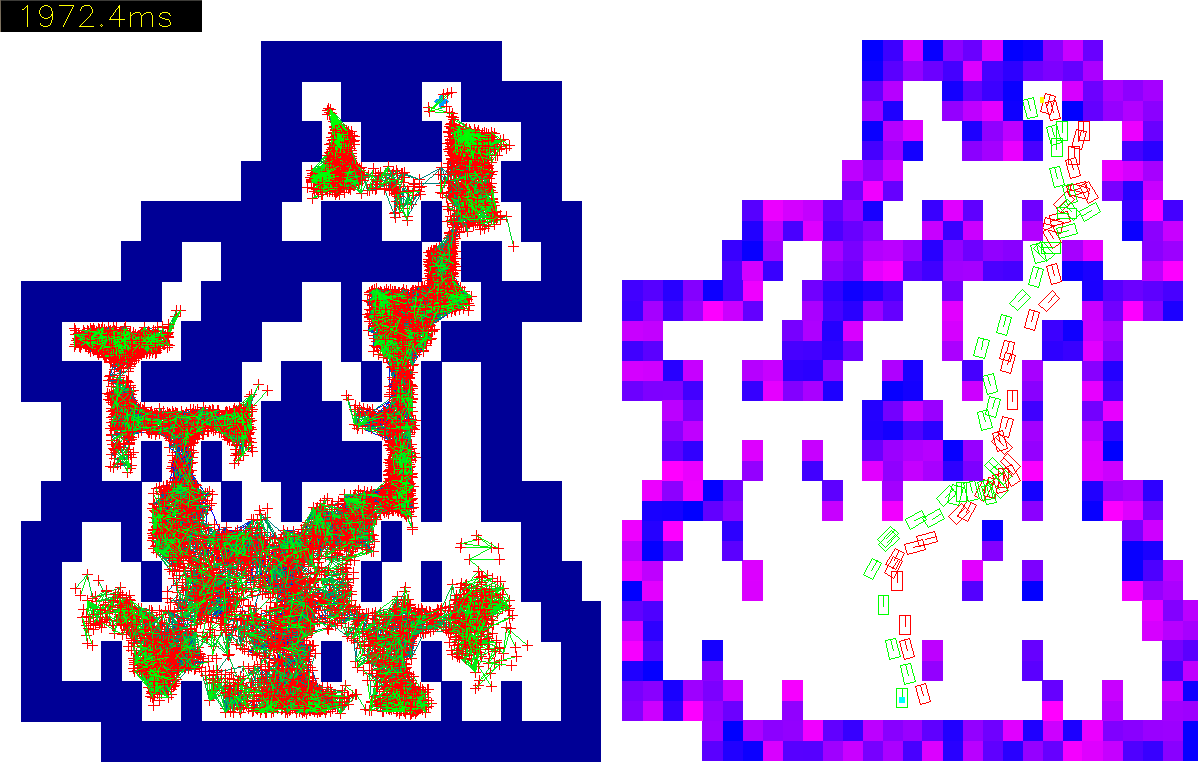
\includegraphics[width=17.0cm]{images/RRT.png}
\caption{A gauche : Représentation de l'arbre généré par l'algorithme RRT. A droite : Séquence de pas générée à partir de l'arbre.}
\label{fig:RRT}
\end{center}
\end{figure}

Afin de pouvoir naviguer dans des environnements avec des obstacles 2D et des obstacles 3D, nous devons tester les collisions (voir~\ref{sub:PQP}) avant de pouvoir valider un pas choisi aléatoirement par le RRT. Ces tests représentent environ 85\% du temps consacré à la planification.

%% Il existant différents moyens pour trouver des trajectoires, les plus connus\footnote{Wikipedia~:~\emph{http://fr.wikipedia.org/wiki/Path-finding}} sont  :

%% \begin{itemize}
%% \item L'Algorithme de Dijkstra~\cite{Dijkstra}, qui permet de déterminer le chemin optimal dans un graphe. Cependant il doit tester un très grand nombre de solutions, il n'est donc pas adapté pour les  grands environnements.
%% \item L'Algorithme A*~\cite{astar} - \emph{a star} - qui est beaucoup plus rapide à condition d'avoir une bonne fonction heuristique, mais qui donne une solution qui n'est pas forcément optimale. En pratique, l'algorithme A* est un bon compromis entre coût calcul et optimalité de la solution.
%% %\item PRM - \emph{Probabilistic RoadMap} - Algorithme en deux étapes, il créé un graphe 
%% \item RRT - \emph{Rapidly-exploring Random Tree} - Cet algorithme de recherche est conçu pour être efficace dans des espaces de grandes dimensions. Un arbre est construit par tirages aléatoires successifs, il s'étend de manière à couvrir rapidement tout l'espace de travail.
%% \end{itemize}

%% Pendant la phase de planification, nous utilisons un version discrète du RRT~\cite{LaValle:WAFR:2000} similaire à celui utilisé dans~\cite{perrin:TRO:2011} pour chercher une séquence de pas faisable.
%% %During the planning phase, we use a discretized version of RRT \cite{LaValle:WAFR:2000} similar to the one used in \cite{perrin:TRO:2011} to search for a collision-free sequence of half-steps.

%% %\vspace{5cm}

%% Les deux premiers algorithmes sont efficaces avec une faible dimension de l'espace des configurations possible. 
%% Dans notre cas, nous utiliserons un ensemble de pas discrets pour le robot, à partir d'un pied d'appui fixe, un ensemble de pas est créé en discrétisant les trois paramètres de configuration $x$, $y$ et $\theta$, ce qui nous donne environ 200 pas faisables.
%% La taille de l'arbre créé par A* croit considérablement avec le nombre de possibilités pour chacun des pas. En général quelques dizaines de configurations sont utilisées pour assurer des temps de génération et de parcours d'arbres assez faibles pour la planification.
%% \vspace{5mm}

%% Afin d'obtenir des replanifications rapides, le temps de recherche du RRT est bridée à $500ms$. Plus l'arbre de recherche est grand, plus le temps passé pour l'étendre est grand (notament la recheche du plus proche voisin présent dans l'algorithme RRT). La figure~\ref{fig:speed} montre le nombre d'itérations effectués par le RRT pendant un laps de temps imparti. La vitesse décroit nettement, c'est pourquoi nous avons choisi de brider la recherche à $500ms$, quitte à faire plusieurs replanifications si aucun chemin n'a pas été trouvé.

%% \begin{figure}[h]
%% \begin{center}
%% 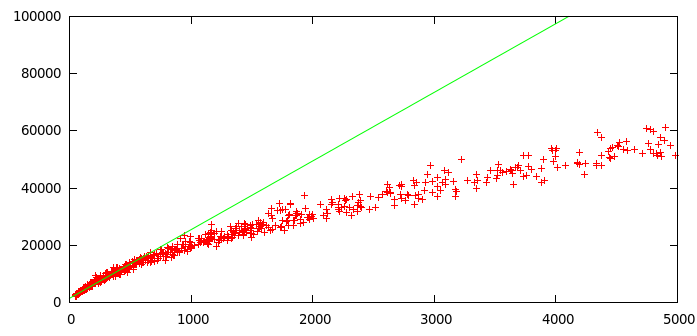
\includegraphics[width=13.0cm]{images/RRT-speed.png}
%% \caption{Nombre d'itérations du RRT en fonction du temps imparti. La droite correspond à l'évolution constatée dans les 500 premières millisecondes.}
%% \label{fig:speed}
%% \end{center}
%% \end{figure}


\subsection{Replanification}
\label{sub:replanif}

%L'objectif de ce stage était de réaliser de la replannification pour le robot HRP-2.
%La première réalisation de cette replannification était de plannifier une trajectoire totale dès qu'un obstacle bouge.

La replanification consiste à trouver un chemin exécutable par le robot afin d'atteindre un objectif tout en évitant, en temps réel, les différents obstacles présents sur son chemin.
%Une des solutions est de rechercher un nouveau chemin dès que quelque chose bouge dans la scène.
Dans l'exemple de la figure~\ref{fig:replan}, la replanification a été nécessaire car un objet a été ajouté sur la trajectoire initiale prévue pour le robot.

\begin{figure}[h]
\begin{center}
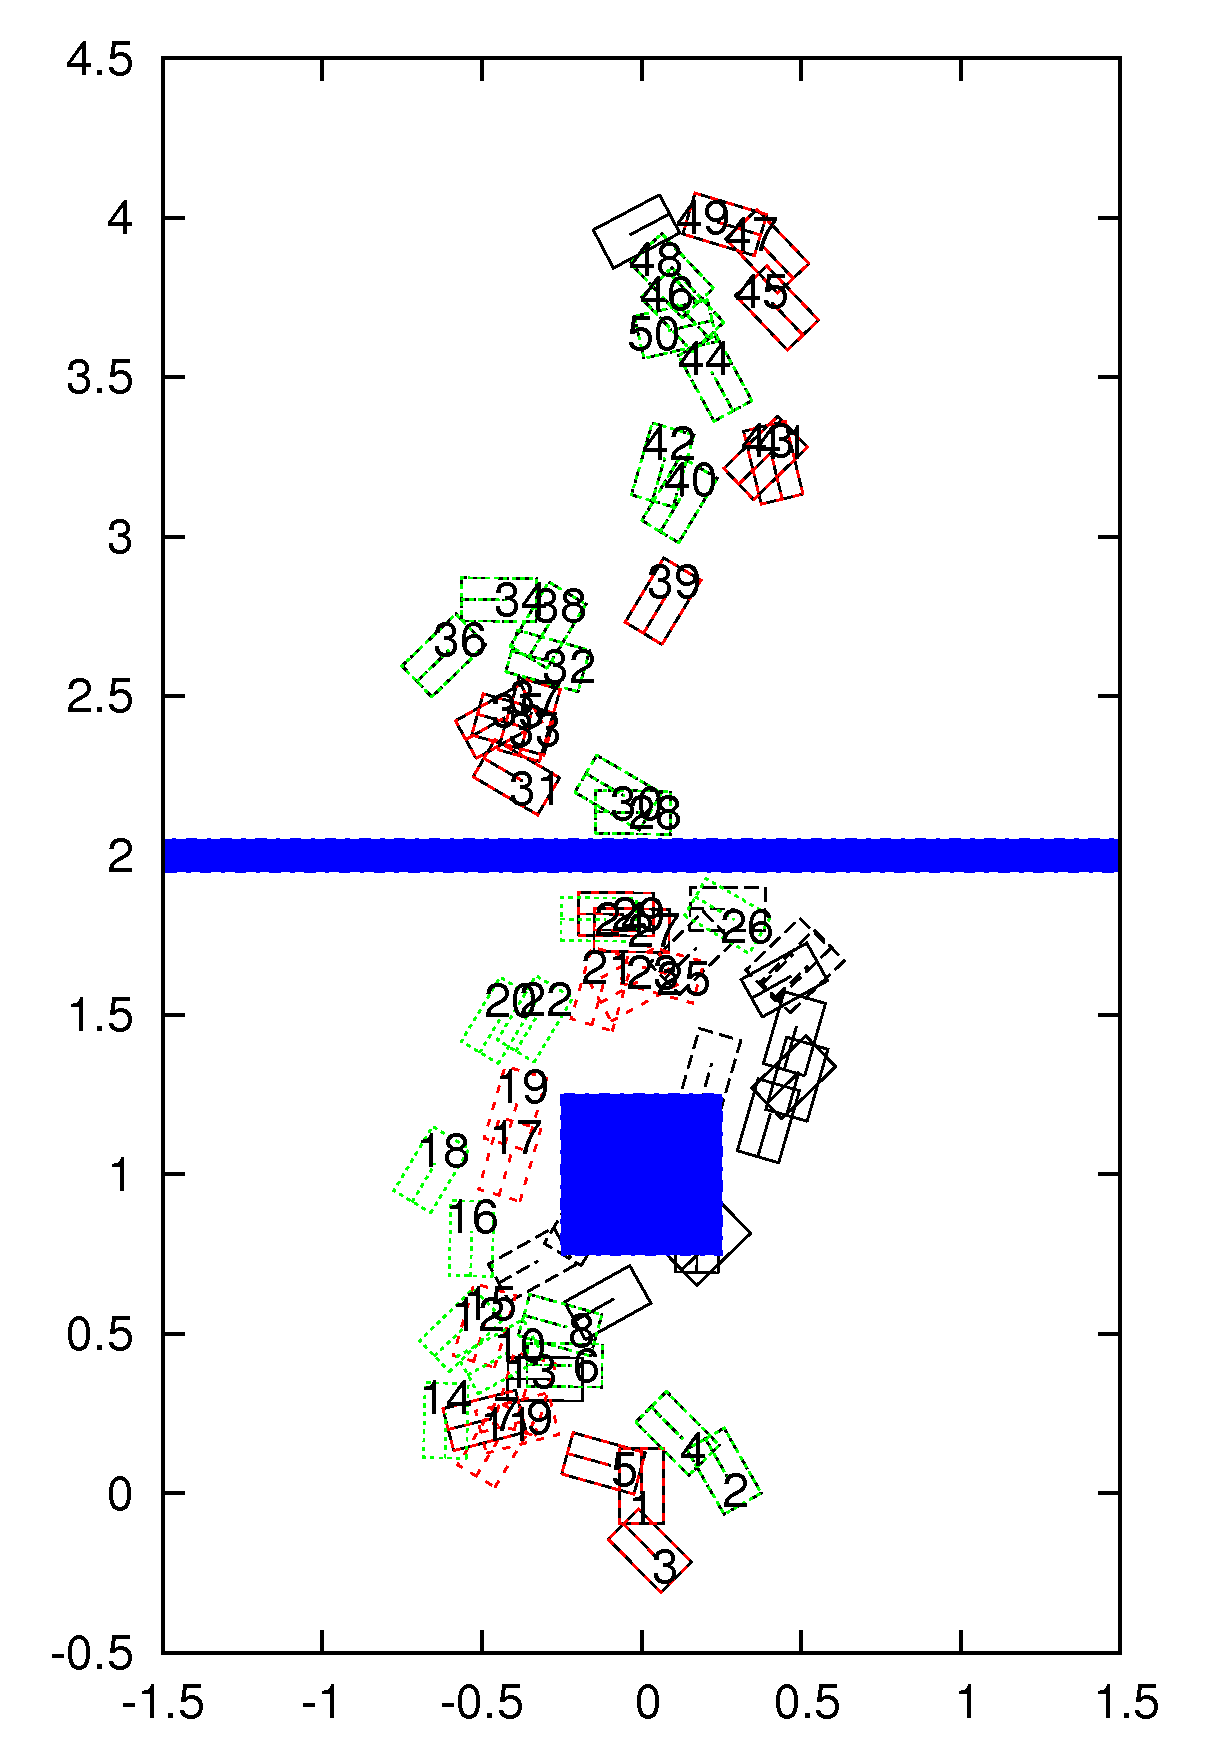
\includegraphics[width=8.0cm]{images/replan.png}
\caption{Exemple d'une trajectoire obtenue après replanification.}
\label{fig:replan}
\end{center}
\end{figure}

Au lieu de replanifier dès qu'un obstacle bouge, le \emph{planner} tente de trouver une nouvelle trajectoire en permanence, en ne gardant la nouvelle que si elle est \emph{meilleure} que la précédente. On va chercher en priorité les trajectoires en marche avant. 

On peut alors dissocier trois cas de figures pour la replanification :
\begin{itemize}
\item Collision avec un obstacle : Ici le robot doit modifier le bout de trajectoire en collision. Pour cela on débute une recherche RRT à partir du pas avant la collision et on définit plusieurs nouveaux objectifs, le but principal, mais également tout les pas après la collision. Si un des objectif est atteint par le RRT nous sommes certains que le robot pourra atteindre l'objectif principal en évitant les collisions.
\vspace{3mm}
\item Objectif modifié : Dans ce cas nous n'avons pas besoin de tout replanifier, en fonction de l'amplitude de la modification on va débuter la recherche RRT à quelques pas de l'objectif (si elle est faible). Sinon on va rechercher un chemin à partir d'une position future du robot afin d'éviter de faire des détours inutiles par l'ancien objectif. On prendra en général trois pas afin de lui laisser le temps nécessaire pour trouver un chemin.
\vspace{3mm}
\item Rien n'a changé : Dans ce cas on va juste faire de l'optimisation de trajectoire. En prenant une position de départ en aléatoire parmi les pas prévus du robot, puis un objectif également dans la liste de pas, on va refaire une recherche de chemins en ne gardant le nouveau chemin que s'il est plus court ou si les pas sont plus majoritairement en marche avant. Pour cela on peut pondérer les pas, un pas en avant va avoir un coût de 1 alors qu'un pas en arrière aura un coût de 2, puis la comparaison de deux trajectoires va revenir à sommer ces poids sur toute la liste de pas.

\end{itemize}


Il arrive que les pas tirés en aléatoire empêchent le robot de franchir un obstacle, il pourra donc prendre plusieurs dizaines de seconde avant de retirer des configurations lui permettant de le franchir. Dans le cadre de la replanification nous ne pouvons pas nous permettre d'attendre indéfiniment que le RRT trouve un chemin. C'est pourquoi nous avons bridé le temps de recherche du RRT à $500ms$, quitte à faire plusieurs planifications si aucun chemin n'a été trouvé pendant le temps imparti.

\subsection{Détection de collision}
\label{sub:PQP}

Pour obtenir une planification de pas en temps réel, nous avons besoin d'effectuer des contrôles de collision très rapides.
Pour ce faire, nous utilisons une approche similaire à celle introduite dans \cite{perrin:TRO:2011} où des approximations des volumes balayés sont précalculées \emph{offline}.

Le principe suit la remarque suivante : après le processus de lissage, la trajectoire finale d'un pas ou d'un demi-pas du robot dépend de nombreux paramètres (paramètres de lissage et les paramètres du pas courant et du pas suivant), \emph{mais avant le lissage}, lorsque la séquence de demi-pas est "brute", la trajectoire du robot ne dépend localement que des paramètres de l'actuel demi-pas.
Les demi-pas ont une propriété intéressante, ils nécessitent seulement trois paramètres pour être complètement définis.
En raison de la basse dimensionnalité de cet espace des paramètres, il est possible d'obtenir une couverture assez dense de l'ensemble des pas réalisables avec seulement un nombre limité de demi-pas fixes.
Nous décidons d'un ensemble fini de demi-pas à l'avance (environ 200), et nous n'utiliserons que ces demi-pas pour produire des séquences de marche.
%Il existe deux types de demi-pas (voir \cite{perrin:TRO:2011}): ascendant et descendant, et avec $N$ demi-pas vers le haut et $N$ demi-pas vers le bas, il est possible de généré $N\times N$ différents pas unique.
Ceci nous donne plus de libertés par rapport aux méthodes où seulement 15 à 30 pas sont considérés \cite{Chestnutt:ICRA:2005,Chestnutt:IROS:2009}.


Une fois l'ensemble fini de demi-pas choisi, pour chacun d'eux nous créons l'approximation du volume balayé par la totalité du corps du robot (voir figure~\ref{fig:SV}), ceci permettra par la suite d'avoir des tests de collisions très rapides.

\begin{figure}[h]
\begin{center}
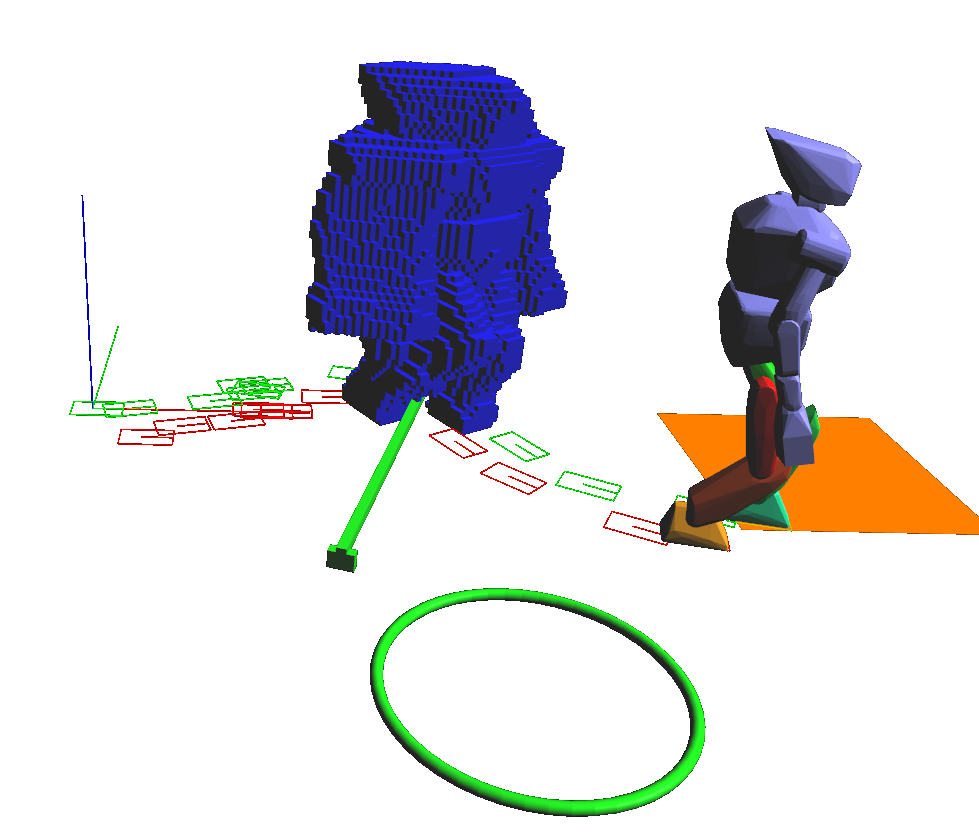
\includegraphics[width=10.0cm]{images/newSweptVolumes.png}
\caption{Approximation du volume balayé par le corps du robot pendant un pas.}
\label{fig:SV}
\end{center}
\end{figure}

Dans~\cite{perrin:TRO:2011}, les approximations des volumes balayés sont stockées dans des structures d'arbres et conçues pour être efficaces avec des environnement définis sous forme de points, mais dans notre implémentation, nous utilisons des arborescences construites à l'aide de PQP~\cite{Larsen:ICRA:2000} à partir d'une \emph{soupe} de triangle.
PQP a l'avantage de détecter les collisions très rapidement à l'aide d'une décomposition en sphère faite lors du chargement du modèle 3D. Nous avons donc, en contrepartie de sa rapidité, un temps mort d'environ une à deux minutes de chargement au début des expériences.


\subsection{Connection de trajectoire}
\label{sub:connection}

A plusieurs occasions nous allons devoir connecter deux trajectoires entre elles : par exemple lorsque le planificateur essaie d'optimiser certaines parties du chemin actuel, il utilise des objectifs intermédiaires. 
Le processus de planification ne pourra jamais tomber exactement sur l'objectif intermédiaire, on doit donc définir si la configuration finale est \emph{assez proche} pour déterminer si l'objectif est atteint ou non.
Dans ce cas, la séquence de pas doit être liée à la précédente, il faut donc ajuster le dernier demi-pas afin de retomber exactement sur l'objectif.
 Cette situation est illustrée sur la figure~\ref{fig:connection}, où le (demi-)pas 102 doit être modifié. 

\begin{figure}[h]
\begin{center}
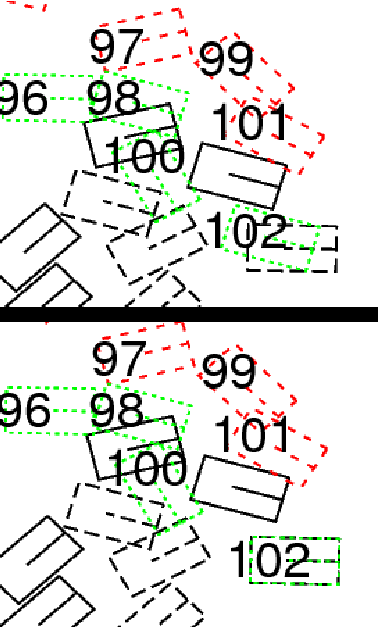
\includegraphics[width=6.0cm]{images/connection.png}
\caption{Connection d'une nouvelle trajectoire au niveau du pas 102. L'image du haut représente la nouvelle trajectoire avant la connection.}
\label{fig:connection}
\end{center}
\end{figure}



Pour savoir comment les pas peuvent être modifiés, nous utilisons de nouveau la propriété de basse dimensionnalité des demi-pas : 
\emph{offline}, nous utilisons des simulations étendues pour décider d'une approximation de la région continue des demi-pas faisables (les demi-pas faisables doivent éviter les auto-collisions et les violations de limites articulaires). 
Grâce à la basse dimensionnalité de l'espace des paramètres pour la définition des demi-pas, cette construction peut être faite en quelques heures.

Après la légère modification du demi-pas il n'appartient plus à l'ensemble fini des demi-pas pour lesquels nous avons une approximation des volumes balayés qui permettent de détecter les collisions (voir \ref{sub:PQP}). Il faudra donc vérifier les collisions avec l'environnement, les dépassements de valeurs articulaires ainsi que les auto-collisions avant de pouvoir valider la modification apportée.





%Résumons encore une fois le processus:
%\begin{itemize}
%\item Nous avons d'abord le plan d'une collision sans marcher séquence de marche en utilisant seulement un nombre fini demi-étapes (phase de planification).
%\item Pour chaque demi-étape, nous savons une approximation conservatrice du volume balayé par le robot durant cette demi-étape, les approximations sont calculées hors ligne.
%Ainsi, nous gagnons beaucoup de temps lors des contrôles de collision: en effet, au lieu d'effectuer des vérifications de collision de nombreux long de la trajectoire à mi-étape, nous effectuons simplement une collision vérifier avec le rapprochement volume balayé.
%\item Une fois une séquence sans collision d'un demi-étapes a été trouvée, nous pouvons commencer à le lisser.
%Cependant, le lissage de la trajectoire correspond à une imprévisible et non défor-mations: nous avons besoin pour faire des contrôles de collision à nouveau. Pour ces tests de collision, nous utilisons l'algorithme PQP avec des représentations des corps convexes robot (il réduit le nombre de triangles).
%Bien sûr, vérifier une trajectoire de collision avec ces vérifications est plus lente qu'avec les approximations volume balayé, mais dans l'ensemble du processus de lissage est beaucoup plus rapide que la phase de planification: en effet lissage se fait uniquement pour l'optimisation de la trajectoire et il n'a pas besoin de considérer des milliers de trajectoires comme le processus de planification.
%\end{itemize}


%% La figure~\ref{fig:scheme} résume le fonctionnement global de la replanification dans le notre cas.
%% \cite{Yoshida:ICRA:2011}
%% \begin{figure}[h]
%% \begin{center}
%% 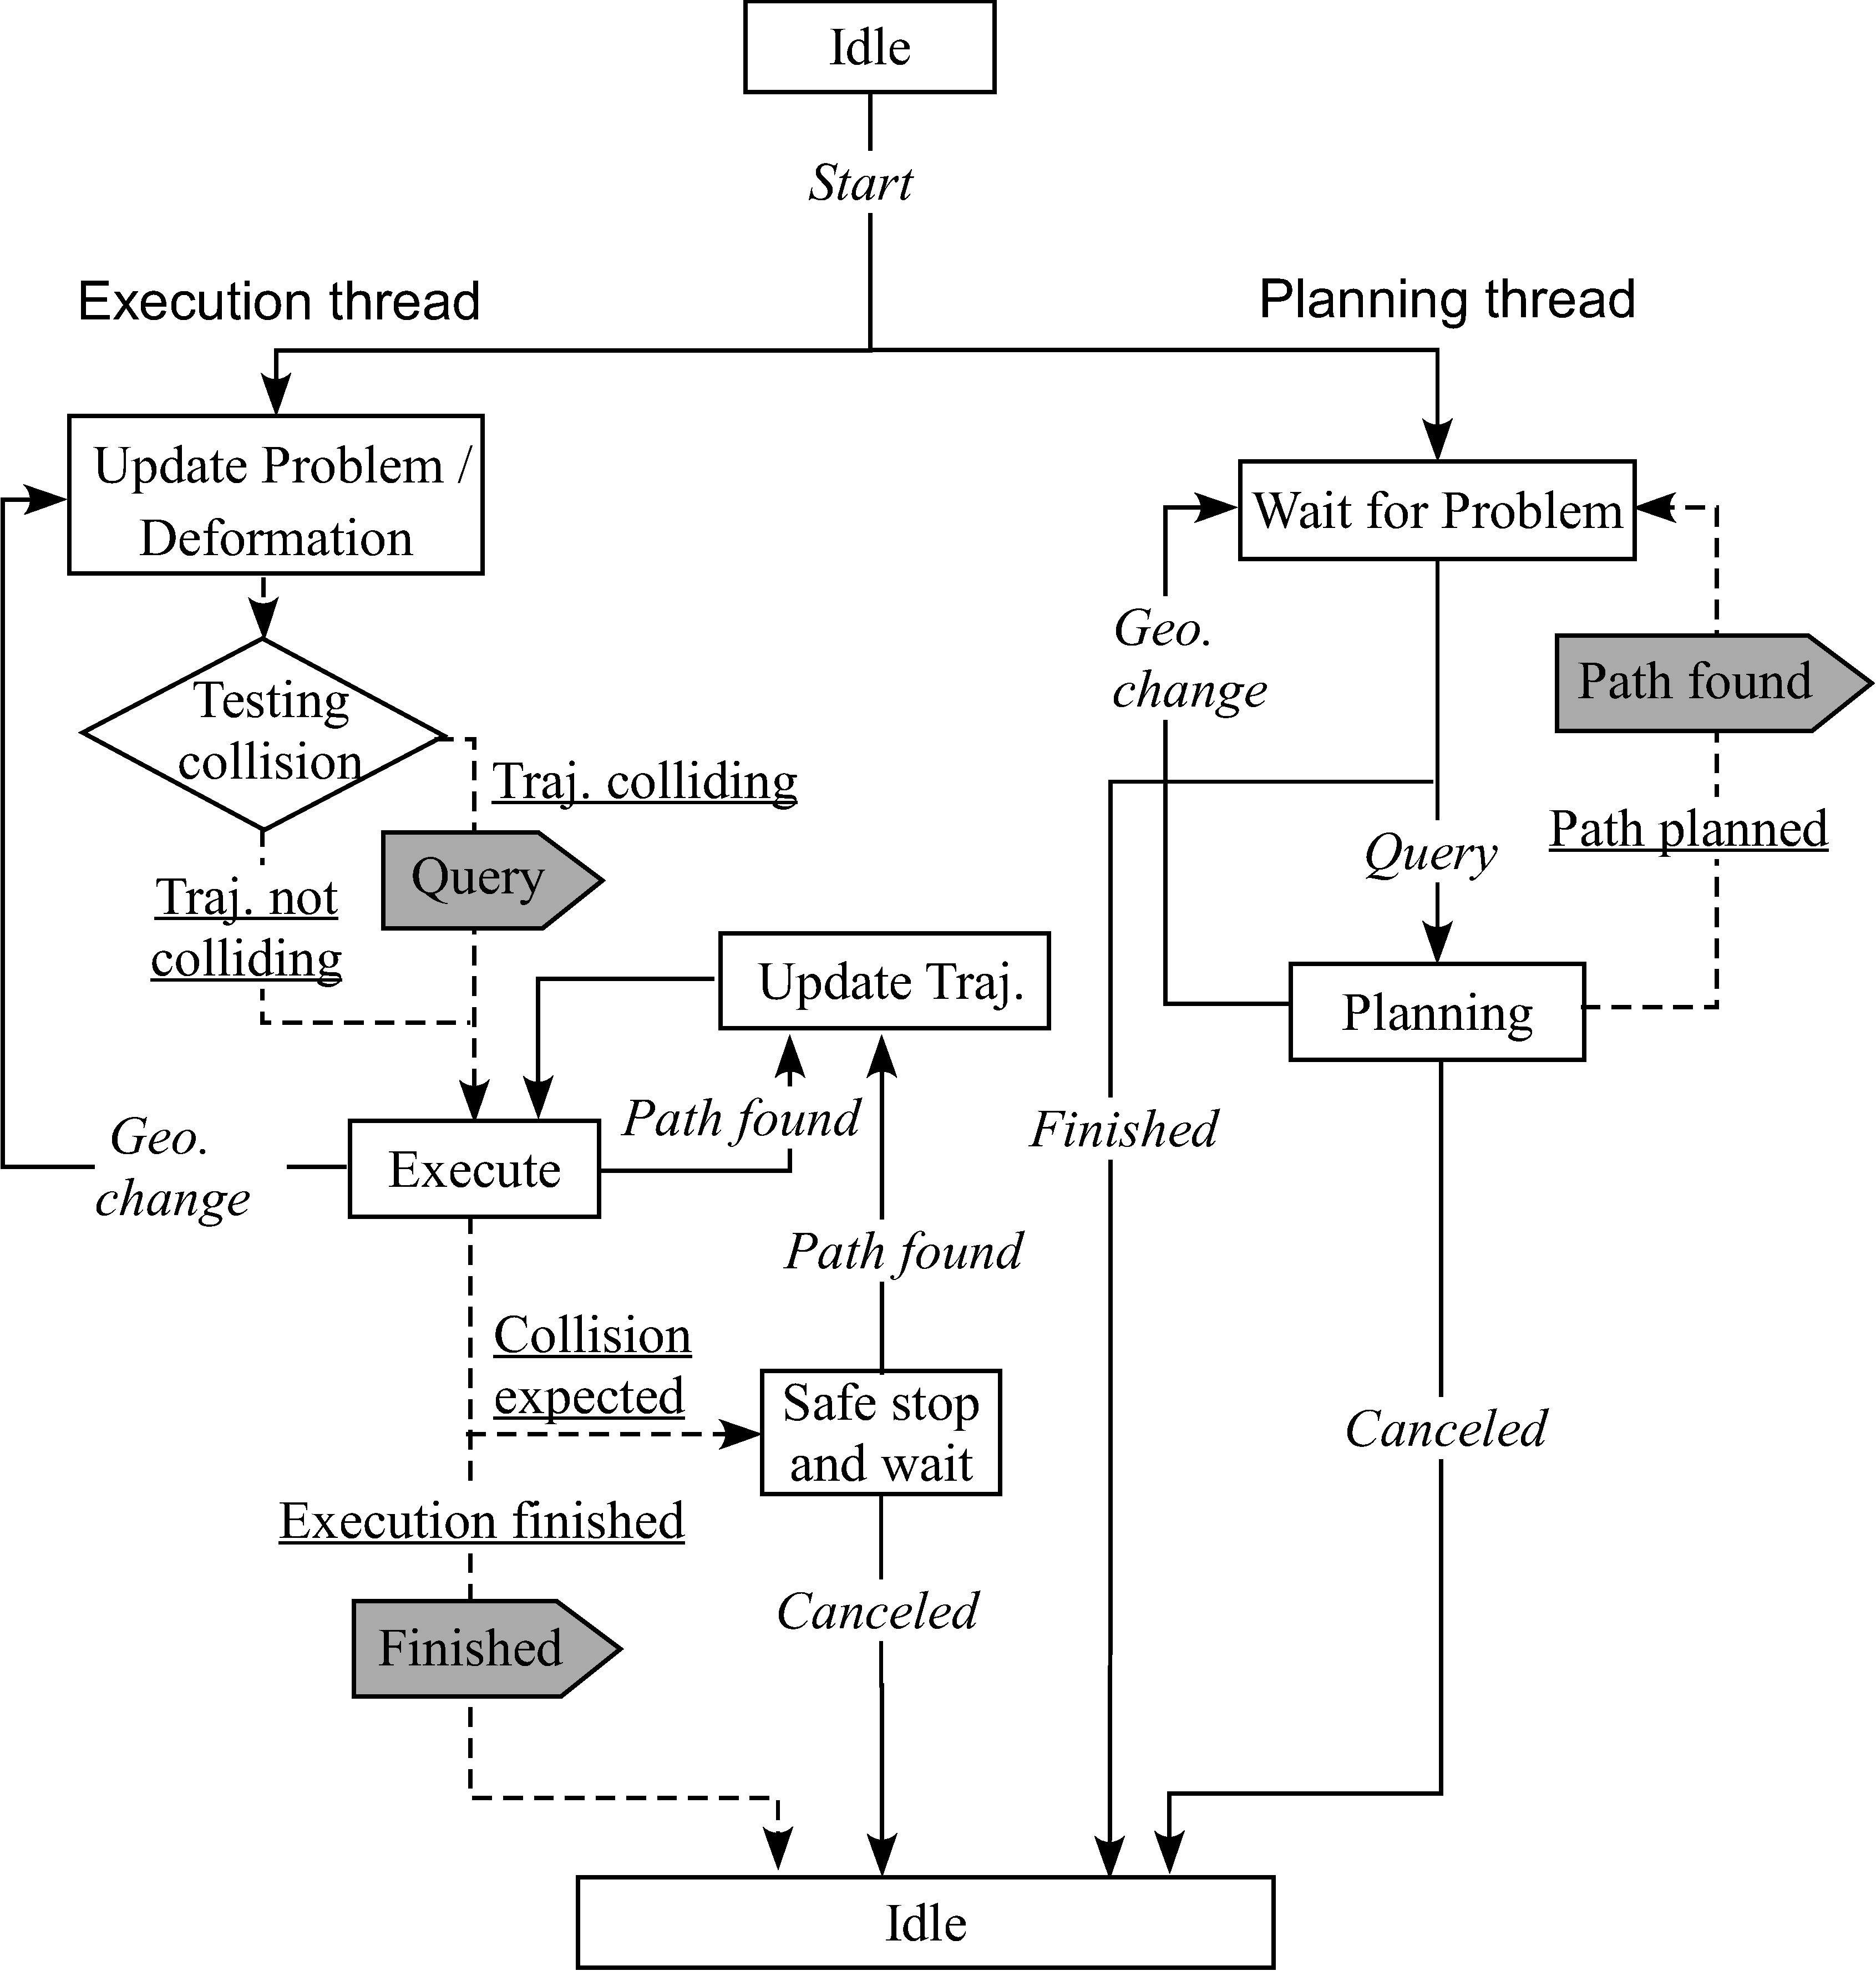
\includegraphics[width=8.0cm]{images/KIR-scheme.png}
%% \caption{Principe général de la replanification.}
%% \label{fig:scheme}
%% \end{center}
%% \end{figure}

%\subsection{Homotopy}
% Once the foot-prints have been decided, the appropriate set of ZMP and CoM trajectories
% has to be found to maintain balance. There is a large body of work dealing with this 
% problem \cite{Kajita03bipedwalking,Nishiwaki:IJRR:09,Morisawa:ICRA:2007}. All those methods
% relies on the Linearized Inverted Pendulum Model relating CoM and ZMP in a simple equation:

\newpage
